\section{Derniers préparatifs}

11 oct. 2009

\begin{multicols}{2}

Bonjour à tous !!

C'est reparti pour un tour, je m'envole pour l'Amérique latine cette fois pour aller découvrir la culture Inca et les beaux paysages de la Cordillère des Andes. A l'heure où je vous écrit, il est 21h, dimanche soir et je décolle demain matin à 10 heure pour une boucle de 5 semaines essentiellement au Pérou et en Bolivie, mais rien n'est réellement fixé et il se peut très bien que j'aille faire un petit tour au Chili, en Argentine, au Paraguay ou au Brésil. En fait le choix se fera réellement sur place, en fonction des rencontres, et peut-être aussi des mouvements sociaux (l'Est de la Bolivie est parfois à éviter), je me renseignerai sur place.

Alors sur une carte, ça donne quoi ?

\smallbreak
\hspace*{-0.65cm}
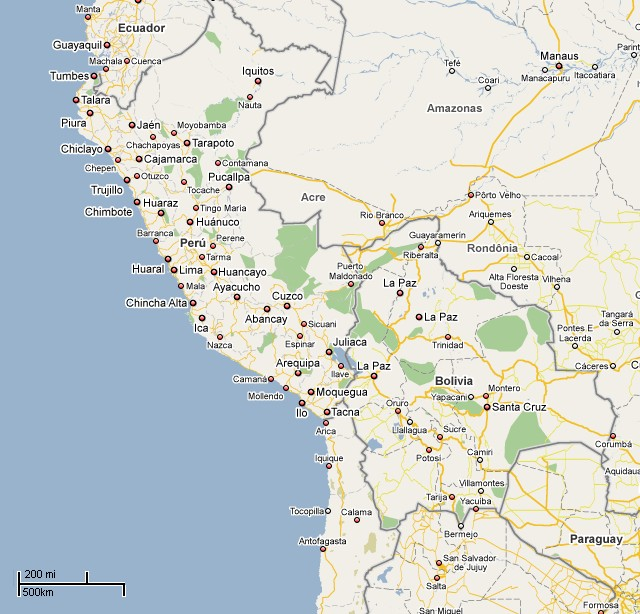
\includegraphics[width=5cm]{articles/Derniers-preparatifs/1255286224vDMd.jpg}
%Carte du Pérou.
\smallbreak

J'atterris à Lima mardi matin, à l'aube (ma journée de lundi aura duré 31h), de là je pars vers le sud par la côte, et je pense m'arrêter à Pisco, juste au dessus de Ica. Et la s'arrêtent les plans, vous lirez la suite ici car je ne la connais pas encore...

Allez, si, j'ai deux destinations à aller voir : Le Machu Pichu, situé près de Cuzco et à une altitude telle qu'il faut du temps pour s'y habituer, puis le Salar Uyuni (désert de sel) situé au Sud de la Bolivie, au Sud Ouest de Potosi.

Sur ce je vous dit à bientôt ici même, j'essaierai de mettre un article toutes les semaines environs (sous réserve de cyber cafés disponible).

Etienne.

\end{multicols}

\bigskip
\textbf{\textsc{Commentaires}}

\medskip
Sam a écrit le 11 oct. 2009 :
\begin{displayquote}
Bon voyage! J'ai hate de lire la suite de tes aventures, petit chanceux !
\end{displayquote}

\medskip
Pegg a écrit le 11 oct. 2009 :
\begin{displayquote}
et seras tu accompagné ? Have a good trip :)
\end{displayquote}

\medskip
Ahlem a écrit le 11 oct. 2009 :
\begin{displayquote}
Ca y est c'est le départ?!
Génial, je suis sûre que ça va être super bien cette "escapade latine".
Bon voyage et amuses toi bien!!!
Ahlem
\end{displayquote}

\medskip
Abanon a écrit le 11 oct. 2009 :
\begin{displayquote}
Bon voyage ! profites en bien !
\end{displayquote}

\medskip
Jaco a écrit le 12 oct. 2009 :
\begin{displayquote}
Enfoiré :)
\end{displayquote}

\medskip
Nicoz a écrit le 12 oct. 2009 :
\begin{displayquote}
Bon voyage et profite bien !
\end{displayquote}

\medskip
Cécile a écrit le 12 oct. 2009 :
\begin{displayquote}
Hé hé, bon voyage! :D
\end{displayquote}

\medskip
Etienne a écrit le 13 oct. 2009 :
\begin{displayquote}
Merci pour vos messages ¡¡¡

Ca y est j'ai atterri a Lima, apres une escale a Miami ou j'ai eu le temps d'aller me ballader sur south beach et de tester les transports en commun du coin\dots eh bien y a un truc de clair c'est qu'en France on a pas a rougir de la qualite de nos bus! J'ai eu droit a un petit florilege de tous nos prejuges sur le americains, mais surtout, tous ceux avec qui j'ai discute etaient super sympa..
C'est decide au retour je prevois mon maillot de bain dans le petit sac cette fois pour aller me baigner entre les deux avions.
Peggy, je suis parti seul.. on prend le meme et on recommence :)
A bientót
\end{displayquote}

\medskip
Philippe a écrit le 14 oct. 2009 :
\begin{displayquote}
Rhâââ\dots Tu n'as pas prévu de maillot de bain pour les sources thermales au pied du Machu Pichu ;-)

Have a nice trip!
\end{displayquote}

\medskip
Yohann a écrit le 15 oct. 2009 :
\begin{displayquote}
Et mec, trop cool l'amerique latine. Amuse toi bien. Et si tu passes en patagonie, prend un max de photo, je prévoie d'y aller en janvier, j'pourrais avoir un aperçu :-)
Léchouilles
PS: trop facile l'anti-spam\dots
\end{displayquote}

\medskip
Helene (ta colloc) ;-) a écrit le 15 oct. 2009 :
\begin{displayquote}
Bon, je vois que tu as atterri, c déjà un bon point.
Par contre tu avais juré de nous donner des nouvelles, heureusement qu'on prend les devants.
Ici ca va, entretiens, entretiens, entretiens\dots ca devient presque une routine et Dova comme d'hab, boulot, boulot, boulot\dots
Allez enjoy, et ne nous oublie pas trop vite!
On pense à toi.
Bisous
Les croqueuses du monde (enfin c'est un peu révolu ca!)
\end{displayquote}

\medskip
Dova (ton autre coloc') a écrit le 16 oct. 2009 :
\begin{displayquote}
Holà, holà!

Révolu?! On n'a pas dit notre dernier mot!
En attendant de croquer de nouveaux horizons, on compte sur toi pour nous faire vibrer durant ces 5 semaines\dots
Hasta pronto y cuidado guapo,
Muchos besos de las mujeres de mundo :))
\end{displayquote}

\medskip
Zé a écrit le 16 oct. 2009 :
\begin{displayquote}
Como estàs Etienne? disfrutando me imagino\dots
Profite bien señor! J'attends la suite avec impatience!
Hasta luego!
\end{displayquote}

\medskip
Dodo a écrit le 18 oct. 2009 :
\begin{displayquote}
Ouaich mon Dud, fait toi bien plaisir, c'est tout ce que je te demande !! En Inde tout s'est super bien passé c'était de la boulette à 7 ! On a souvent pensé à toi\dots Et tes biddies attendent sagement
La bise
\end{displayquote}

\medskip
Helene (ta colloc) ;-) a écrit le 20 oct. 2009 :
\begin{displayquote}
Salut!
Bon alors, c qd que tu le remets à jour ton blog????
Bz
\end{displayquote}

\vfill

